%!TEX root = Lefley - Mesh to voxel transformations for optimised physics-based interactions.tex
\chapter{Preparation}

This chapter will detail the planning and preparation done before the project was undertaken. The refinement of the original idea, as found in the project proposal, as well as the necessary groundwork undertaken will be discussed.

\section{Refinement}

This project has the aim to investigate a new approach to resolving physically induced damage in objects. However, the term damage encompasses a wide range of processes. Furthermore there are many stimuli that could result in physical damage occurring.

It was decided that the scope of this project would be limited to fragmentation as a form of damage. We define fragmentation to be the partitioning of a rigid solid into smaller rigid solids, assumed to be made of the same material as the original object. This process should conserve mass as much as possible, with no loss between the original object and sum of the resultant fragments. 

The physical stimulus that this project is constrained to is collision. We focus on simple collisions between two discrete objects where only one object is capable of fragmenting. We use relevant information from the collision such as object masses and impact velocities and use it to construct as accurate an outcome as possible, including ensuring each fragment has an accurate movement vector post collision.

While the simulation conditions have been constrained for the scope of this project, the principle of computing an object's volume in order to accurately simulate the destruction of that object is transferable to wider conditions.

\section{Resources Used}

Unity3D was used as a basic engine with which to work. The engine provided general features such as rendering, rigid mesh physics and game object management which were expanded upon to achieve the more specific required goals. As Unity3D is a widely used commercial engine, any time or space overheads introduced by the engine can be more safely ignored in analysis as they would also be present in other solutions. There also exist other object destruction libraries written for the engine which have been used for comparative evaluation\cite{Meshinator}.

A {\sc{HLSL}} DirectCompute shader implementing the Schwartz method for solid voxelisation, found in GPU Pro 3 has been adapted for use and a {\sc{C\#}} driver written\cite{Schwarz:2010:Vox}\cite{Engel:2012:GPA:2331213}. The original library had a {\sc{C++}} driver which handled both the setup and dispatch of the shader as well as rendering. The methods regarding setup and dispatch were analysed and their functionality reproduced in {\sc{C\#}} using Unity library calls for invoking dispatches.

An existing implementation of the marching tetrahedra algorithm on the CPU for voxel to mesh transformations\cite{Tetrahedra-CPU} was used. The original library generated a 3D scalar field from perlin noise and then used this to implicitly define a surface which was then meshed using marching tetrahedra. The perlin noise generating code was removed and the 3D field used by the marching tetrahedra methods exposed as an input.

\section{Required Understanding}

The majority of code for this project was written in {\sc{C\#}}, a language which required some learning.

\subsection{Voxelisation}

In order to write a driver for the GPU implementation of solid binary voxelisation found, both the method and shader language used had to be understood. The description of the algorithm featured in GPU Pro 3 was read and a tutorial for HLSL, particularly its use with Unity3D, followed\cite{Engel:2012:GPA:2331213}.

\subsection{Fragmentation}

An understanding of basic physics was required for the resolution of damage as described. This was to ensure that the outcome was as accurate as possible under the involved forces and defined object properties. As the project is more focussed on the Computer Science aspects of this method of damage resolution, the physics calculations used are not so complicated as to truly simulate the real world.

Voronoi methods for fracturing were also studied as these are what are most commonly used for fragmentation in simulations. This is because they produce results that are dynamic rather than predefined\footnote{See Section~\ref{sect:relfrag}.} and are efficient\cite{Muller:2013:RTD:2461912.2461934}.

\subsection{Meshing}

The marching tetrahedra algorithm was studied for use forming the implicit surfaces defined by the voxels in each fragment. Both a GPU and CPU implementation were found and explored. The CPU implementation was found to be sufficient and used as a starting point for the meshing phase of the pipeline\cite{Tetrahedra-CPU}.

\section{Requirements Analysis}

\label{sect:req}

In order for the project to be considered successful in investigating a new approach for object damage it was decided that the following should be met:

\begin{itemize}
\item{The solution \emph{must} enable a scene in which an object with up to 65,534 vertices\footnote{The limit imposed by Unity3D} is fragmented in a manner which resembles a real world interaction as closely as possible.}
\item{The solution \emph{must} be object independent. That is any object may be made destructible without retroactively altering the object's definition.}
\item{The solution \emph{must} take into account the defined physical characteristics of the object to be fragmented as well as those defined by the collision when resolving.}
\end{itemize}

\begin{itemize}
\item{The solution \emph{should} produce fragments with the correct physical properties based on those of the original object and the size of the each given fragment.}
\item{The solution \emph{should} work with both convex and concave objects.}
\end{itemize}

\begin{itemize}
\item{The solution \emph{could} run in real-time.}
\end{itemize}

\begin{itemize}
\item{The solution \emph{won't} deal with texture mapping onto fragments.}
\item{The solution \emph{won't} deal with structural integrity.}
\end{itemize}

\section{Planning}

\subsection{Pipeline}

As detailed previously, the destruction process was split into three sections:

\begin{enumerate}
\item{Voxelisation}
\item{Partitioning}
\item{Remeshing}
\end{enumerate}

It was decided what each section should input and output ahead of time to ensure two things.

\begin{itemize}
\item{Different implementations of each section could be easily interchanged.}
\item{Each section would output something that allowed for easy testing of that section.}
\end{itemize}

Figure~\ref{fig:2.1} illustrates this decision.

\begin{figure}
\centerline{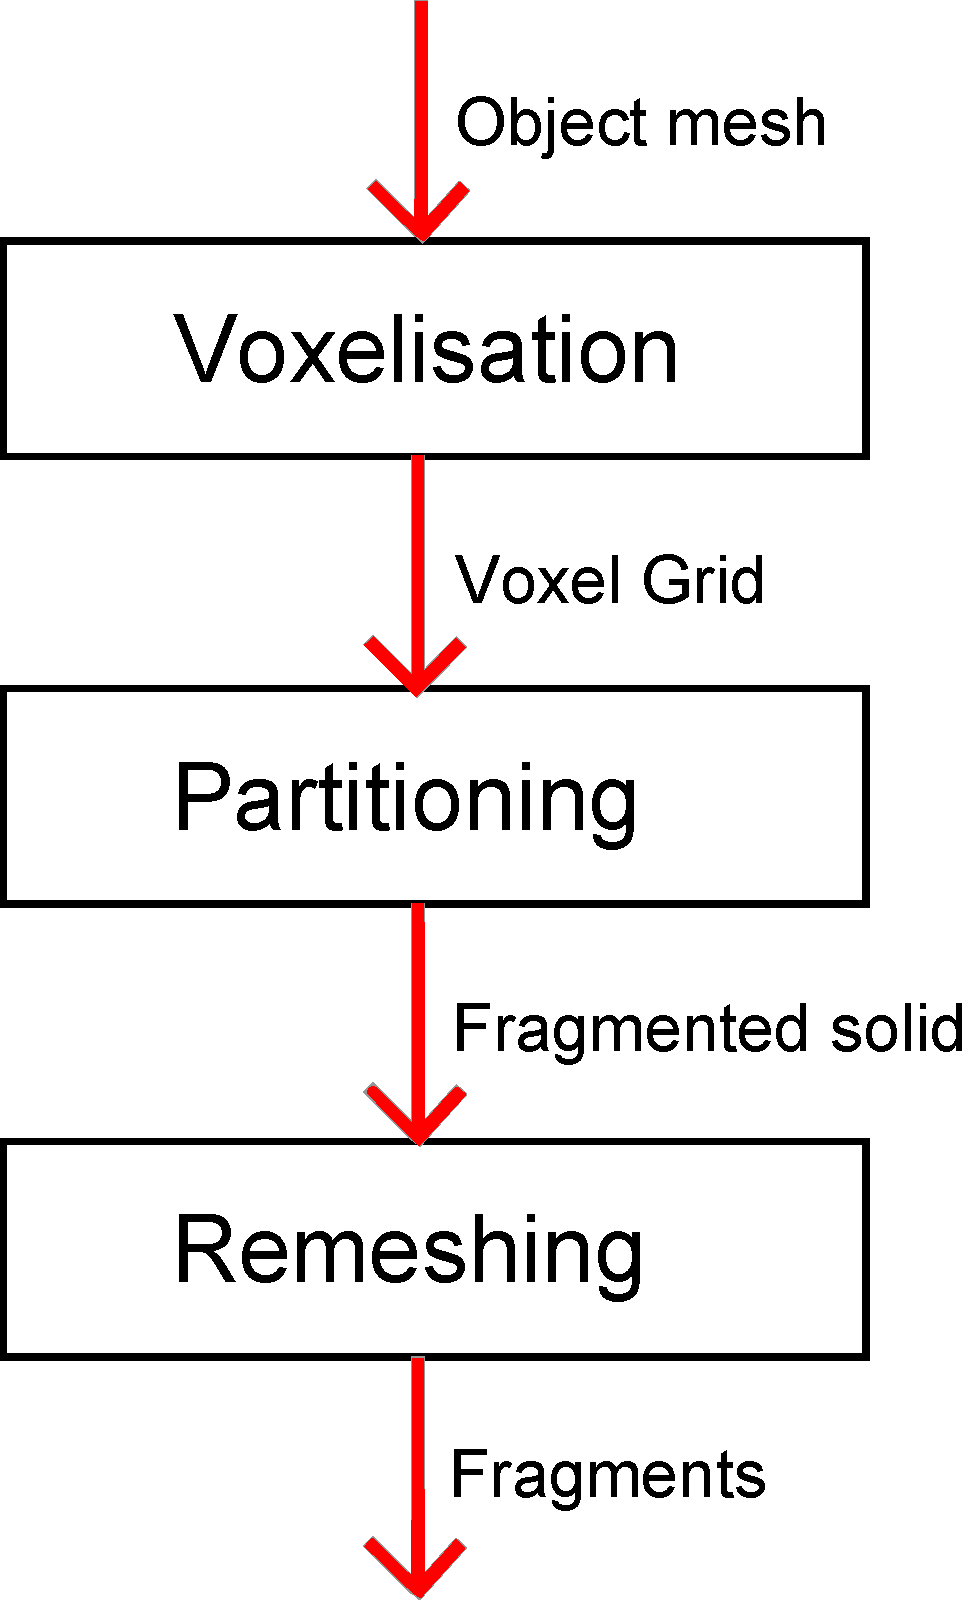
\includegraphics[scale=0.3]{pipeline13.pdf}}
\caption{The proposed pipeline.}
\label{fig:2.1}
\end{figure}

\subsection{Class Structure}

%Based on the above description of the pipeline the following class structure was used.

The decision was made to have driver classes which processed the inputs and outputs to their respective implementation of a pipeline stage. An overarching driver would then manage the passing of output to input between drivers, doing any intermediate data processing required. A delegating driver managing all of the pipeline stage drivers rather than an actual pipeline of driver was chosen as it allows for easier manipulation of data between stages as well as debugging. Switching out different implementations of the stages also becomes easier.

\section{Conclusion}

In order for the implementation of the proposed solution to run smoothly and the requirements to be achieved, it was necessary to become familiar with the technologies, languages and algorithms to be used. The most important part of preparation was devising the pipeline and investigating the existing solutions for the required work in each stage. This was so that implementation could proceed in a sequential manner through the pipeline with knowledge of the upcoming stages allowing for correct design.